\documentclass[aspectratio=43]{beamer}

% packages
\usepackage{unicode-math}

% use cambridgeUS theme with beaver colors
\usetheme{CambridgeUS}
\usecolortheme{rose}

% presentation information%
\title{Introduction to Differential Privacy}
%\subtitle{Differential Privacy in Distributed Settings}
\date{November 14, 2019}
\author[Bj\"orn Bebensee]{Bj\"orn Bebensee \\ {\tt bebensee@bi.snu.ac.kr}}
\institute[Seoul National University]{{\normalsize Seoul National University}}

% set the logo
%\logo{
\includegraphics[width=0.2\textwidth]{fig/bi.png}}

% set left and right margins
\setbeamersize{text margin left=12mm,text margin right=12mm}

% remove navigation symbols
\setbeamertemplate{navigation symbols}{}

% use unicode
\usepackage[utf8]{inputenc}

% use tikz
\usepackage{tikz}

%custom footline
\setbeamertemplate{footline}
{
  \leavevmode%
  \hbox{%
  \begin{beamercolorbox}[wd=.333333\paperwidth,ht=2.25ex,dp=1ex,center]{author in head/foot}%
    \usebeamerfont{author in head/foot}\insertshortauthor
  \end{beamercolorbox}%
  \begin{beamercolorbox}[wd=.333333\paperwidth,ht=2.25ex,dp=1ex,center]{title in head/foot}%
    \usebeamerfont{title in head/foot}\insertshortinstitute
  \end{beamercolorbox}%
  \begin{beamercolorbox}[wd=.333333\paperwidth,ht=2.25ex,dp=1ex,right]{date in head/foot}%
    \usebeamerfont{date in head/foot}\insertshortdate{}\hspace*{2em}
    \insertframenumber{} / \inserttotalframenumber\hspace*{2ex} 
  \end{beamercolorbox}}%
  \vskip0pt%
}

\setbeamertemplate{section in toc}[sections numbered]

\begin{document}

%------------------------------------------------
% TITLEPAGE
%------------------------------------------------

\begin{frame}
\titlepage
\end{frame}

%------------------------------------------------
% TABLE OF CONTENTS
%------------------------------------------------

\begin{frame}{Contents}
    \tableofcontents
\end{frame}

%------------------------------------------------

\section{Motivation}

\begin{frame}{Motivation}
    Imagine we have a database of users. We want to publish some anonymous statistics about the users.\\
    \onslide<2->{
    \bigskip
    \textbf{This is a hard problem!}\\
    \bigskip
    Famously researchers uniquely identified 99\% of users in the ``anonymized'' Netflix Prize dataset in 2007.
    }
\end{frame}

%------------------------------------------------

\begin{frame}{Motivation}
    \textbf{Given:} a database of users\\
    \smallskip
    \textbf{Compute:} statistics over all users\\
    \smallskip
    \textbf{Constraint:} protect the information of each single user\\
    \bigskip
    \textbf{Adversary:} Potentially malicious actor who either
    \begin{itemize}
        \item is able to query the \emph{statistical database} (\emph{interactive setting})
        \item only has access to the published statistics (\emph{noninteractive setting})
    \end{itemize}
\end{frame}

%------------------------------------------------

\section{Differential Privacy}

\subsection{Definition}

\begin{frame}{Differential Privacy}
    Differential privacy is a framework of statistical techniques.\\
    It is used to
    \bigskip
    \begin{itemize}
        \item[(1)] compute statistical queries on user inputs
        \item[(2)] protect each individuals' privacy while doing so
    \end{itemize}
    \bigskip
    Allows a trade-off between utility and user privacy.
\end{frame}

%------------------------------------------------

\begin{frame}{Differential Privacy}
    \begin{definition}
        A randomized function $\mathcal{K}$ gives $\epsilon$-Differential Privacy if for all data sets $D_1$ and $D_2$ differing on at most one element, and all $S \subseteq Range(\mathcal{K}),$
        $$
        \frac{\text{Pr}[\mathcal{K}(D_1) \in S]}{\text{Pr}[\mathcal{K}(D_2) \in S]} \leq e^{\epsilon}
        $$
    \end{definition}
    \bigskip
    An algorithm is $\epsilon$-DP if it does not depend on any single entry in the dataset but rather (probably) gives the same output even if you remove any single entry.
\end{frame}

%------------------------------------------------

\subsection{Achieving Differential Privacy}

\begin{frame}{Differential Privacy}
    \centering
    How can we achieve $\epsilon$-Differential Privacy?
\end{frame}

%%------------------------------------------------

\begin{frame}{Differential Privacy}
    \textbf{Idea:} Inject random noise to protect the privacy of individuals.\\
    \bigskip
    Example: What are the number of users with a bad credit rating?\\
    \bigskip
    Ground truth $N=21$, $X$ random variable with Laplace distribution. Return $N+X$.\\
    \onslide<2->{
        \bigskip
        \begin{alertblock}{Problem}
            Privacy losses accumulate. An adversary can estimate the ground truth given enough queries. More queries correspond to laxer privacy guarantees.
        \end{alertblock}
    }
\end{frame}

%------------------------------------------------

\begin{frame}{Differential Privacy}
    To address this define a function's sensitivity as follows:
    \bigskip
    \begin{definition}
        For a function $f: D \rightarrow R^k$, the sensitivity of $f$ is
        $$
        \Delta f = \max_{D_1,D_2} || f(D_1) - f(D_2) ||_1
        $$
        for all datasets $D_1, D_2$ differing in at most one element.
    \end{definition}
    \bigskip 
    Then, for a query function $f$, return
    $$
    f(x) + \mathrm{Lap}(\Delta f / \epsilon)
    $$
    with \emph{privacy loss} $\epsilon$, i.e. the variance depends on the sensitivity and the privacy loss.
\end{frame}


%------------------------------------------------

\subsection{Problems}

\begin{frame}{Problems}
    However, there are some problems with (centralized) DP:\\
    \medskip
    \begin{itemize}
        \item[1.] Still requires trust in a central authority!
        \item[2.] Distributed setting: inputs are connected to identifiers such as IP address in logs etc.
    \end{itemize}
    \onslide<2->{
        \bigskip
        \begin{alertblock}{Goal}
        \begin{itemize}
            \item Compute user statistics in a distributed setting, w/o trust in central authority
            \item Efficient computation, low communication cost (important on mobile devices)
        \end{itemize}
        \end{alertblock}
    }
\end{frame}

%------------------------------------------------

\section{Local Differential Privacy}

\subsection{Randomized response}

\begin{frame}{Randomized response}
    Idea for the distributed setting: randomized response\\
    \bigskip
    \textbf{Survey technique} introduced in 1965 to get accurate statistics on sensitive topics.\\
    \medskip 
    Example: Have you used drugs this month?
\end{frame}

%------------------------------------------------

\begin{frame}{Randomized response}
  \begin{itemize}
        \item[1.] Participants toss a coin
        \item[2.] Answer truthfully if coin comes up heads
        \item[3.] If tails, participant tosses a 2nd coin:
        \begin{itemize}
            \item ``Yes" if tails
            \item ``No" if heads
        \end{itemize}
    \end{itemize}
    \bigskip
    True answer if first coin heads or 50\% chance on second coin. Answer truthfully $\sim$75\% of the time.
\end{frame}

%------------------------------------------------

\begin{frame}{Randomized response: analysis}
    Given positive answers $X$, true number of ``Yes" answers:
    \begin{gather*}
        Y = 2(X-0.25)
    \end{gather*}
    \bigskip
    \textbf{Result:} plausible deniability for participants, accurate statistics
\end{frame}

%------------------------------------------------

\begin{frame}{Local Differential Privacy}
    \begin{figure}
        \centering
        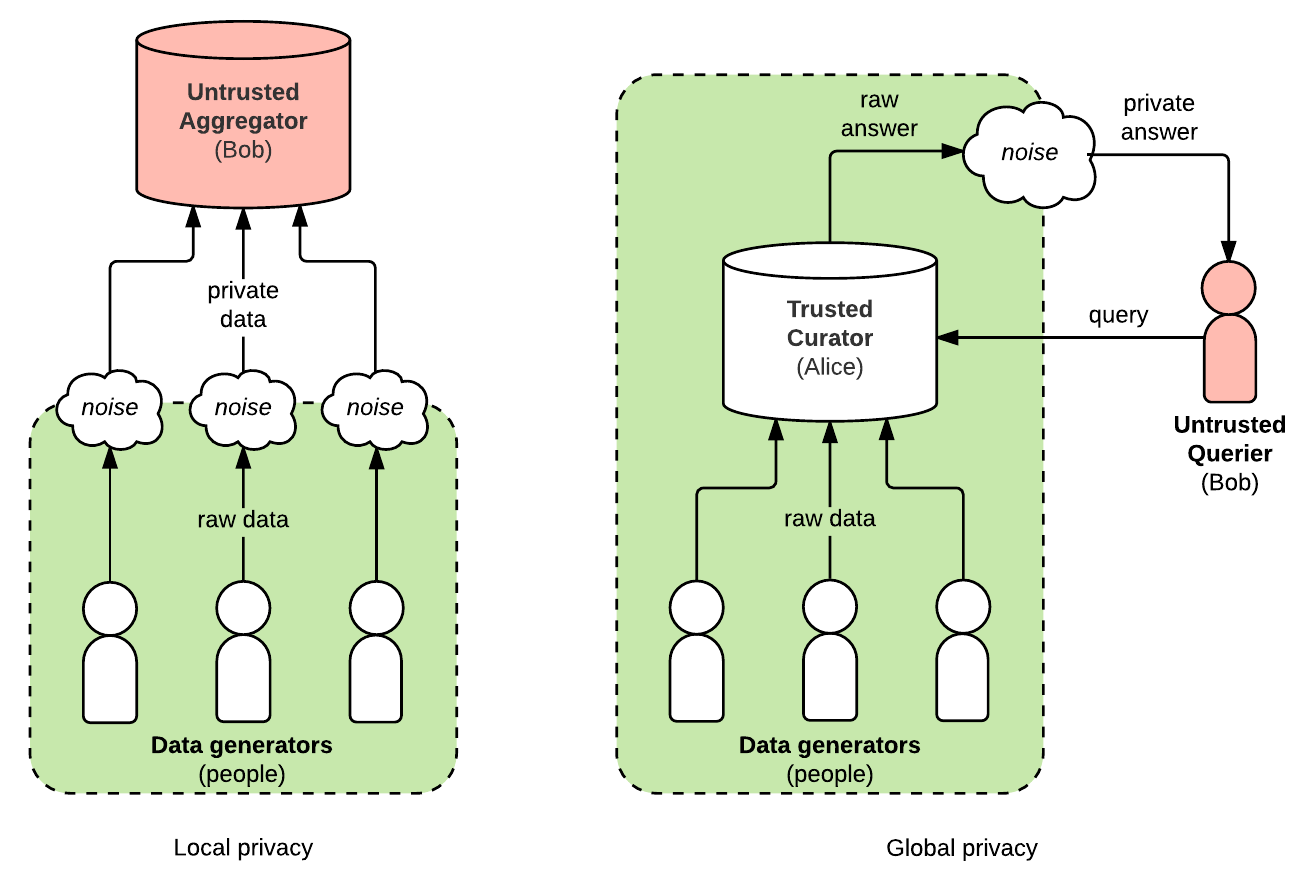
\includegraphics[width=0.9\textwidth]{fig/ldp.png}
        \caption{Local differential privacy vs. differential privacy}
    \end{figure}
\end{frame}

%------------------------------------------------

\subsection{Definition}

\begin{frame}{Local Differential Privacy}
    \begin{definition}
        We say that an algorithm $\pi$ satisfies $\epsilon$-Local Differential Privacy where $\epsilon > 0$ if and only if for any input $v$ and $v'$
        $$
        \forall y \in Range(\pi): \frac{Pr[\pi(v) = y]}{Pr[\pi(v') = y]} \leq e^\epsilon
        $$
        where $Range(\pi)$ denotes every output of the algorithm $\pi$.
    \end{definition}
    \bigskip
    For the randomized response example: survey participants are given $\epsilon$-LDP guarantee with $\epsilon = ln(0.75/(1-0.75)) = ln(3)$
\end{frame}

%------------------------------------------------

\subsection{Challenges}

\begin{frame}{Challenges in the local model}
    \begin{alertblock}{Challenges}
        It is much harder to construct protocols for the local model:
        \begin{itemize}
            \item more difficult to maintain low error-bound
            \item maintain low communication cost (ideally only a few bits)
        \end{itemize}
    \end{alertblock}
    \onslide<2->{
        \bigskip
        \textbf{centralized model}: add Laplace noise of magnitude $O(1/\epsilon)$, independent of number of participants\\
        \medskip
        \textbf{local model}: lower-bound $\Omega(\sqrt{n}/\epsilon)$, dependent on number of participants
    }
\end{frame}

%------------------------------------------------

\section{Key problems in LDP}

\subsection{Overview}

\begin{frame}{Key problems in LDP}
    There are a number of different problems in LDP. We will look at a few of them:\\
    \bigskip
    \begin{itemize}
        \item Frequency estimation
        \item Heavy hitter identification
        \item Private spatial data collection
    \end{itemize}
\end{frame}

%------------------------------------------------

\subsection{Frequency oracles}

\begin{frame}{Frequency Oracles}
    \begin{definition}
        Given a domain $\mathcal{D}$ a \emph{frequency  oracle} (FO) is a protocol which estimates the frequency of an element $d \in \mathcal{D}$.
    \end{definition}
    \bigskip
    Core problem of LDP: locally private frequency estimation
\end{frame}

%------------------------------------------------

\begin{frame}{FO framework}
    Define \emph{pure} FO protocols by a composition of \textbf{encoding} and \textbf{perturbation} and \textbf{support}.\\
    \bigskip
    \textbf{Encoding}: Encoding of each value in the domain $\mathcal{D}$\\
    \bigskip
    \textbf{Perturbation}: Random perturbation of encoded values\\
    \bigskip
    \textbf{Support}: Mapping of each output $y$ to the set of inputs that support the output value $y$\\
    \bigskip
    The true frequency $c(i)$ of a value $i$ can then be estimated given the encoding, perturbation and support.
\end{frame}

%------------------------------------------------

\begin{frame}{Direct Encoding}
    Generalization of randomized response with coin flip.\\
    $\text{Encode}(v) = v$. Perturb with:
    \bigskip
    $$
    \text{Pr}[\text{Perturb}(x) = i] =
        \begin{cases}
            p = \frac{e^{\epsilon}}{e^{\epsilon}+|\mathcal{D}|-1}, & \text{if } i=x\\
            q = \frac{1-p}{|\mathcal{D}|-1} = \frac{1}{e^{\epsilon}+|\mathcal{D}|-1}, & \text{if } i \neq x
        \end{cases}
    $$\\
    \bigskip
    The support function is $\text{Support}_{\text{DE}}(i) = \{ i \}$.
\end{frame}

%------------------------------------------------

%\begin{frame}{Histogram Encoding}
%    For a value $v$ its encoding is a vector of length $|\mathcal{D}|$ in which each entry is 0.0 and only the $v$-th component equals 1.0. It is then perturbed using the Laplace distribution such that $B'[i] = B[i] + \text{Lap}(\beta)$.\\
%    \bigskip
%    \textbf{Aggregation}:\\
%    \bigskip
%    \begin{itemize}
%        \item Summation with Histogram Encoding (SHE): sum up the reported noisy histograms from all users $\Rightarrow$ not a pure protocol
%        \item[]
%        \item Thresholding with Histogram Encoding (THE): interpret each noisy count above a threshold $\theta$ as a 1 and each count below $\theta$ as a 0
%    \end{itemize}
%\end{frame}

%------------------------------------------------

\begin{frame}{Unary Encoding}
    Value $v$ is encoded as a bit vector where only the $v$-th position equals 1 and all other positions equal 0. Given probabilities $p,q$ the perturbed output $B'$ is computed as follows:
    \bigskip
    $$
    \text{Pr}[B'[i] = 1] = 
        \begin{cases}
            p, & \text{if } B[i] = 1\\
            q, & \text{if } B[i] = 0
        \end{cases}
    $$\\
    \bigskip
    with optimal parameters $p = \frac{1}{2}$ and $q = \frac{1}{e^{\epsilon}+1}$ and the support function $\text{Support}_{\text{UE}}(B) = \{ i \ | \ B[i] = 1 \}$.
\end{frame}

%------------------------------------------------

%\begin{frame}{Binary Local Hashing}
%    Universal family of hash functions $\mathbb{H}$, such that each hash function $H \in \mathbb{H}$ hashes an input $d \in \mathcal{D}$ into one bit\\
%    \bigskip
%    Then $\text{Encode}(v) = \langle H, b \rangle$ with $H \in \mathbb{H}$ chosen uniformly at random and $b = H(v)$\\
%    \bigskip
%    Given $\epsilon$, input bit $b$ compute perturbed input $\langle H,b' \rangle$:\\
%    \bigskip
%    $$
%    \text{Pr}[b' = 1] =
%        \begin{cases}
%            p = \frac{e^{\epsilon}}{e^{\epsilon}+1}, & \text{if } b = 1\\
%            q = \frac{1}{e^{\epsilon}+1}, & \text{if } b = 0
%        \end{cases}
%    $$\\
%    \bigskip
%    $\text{Support}_{\text{BLH}}(\langle H,b \rangle) = \{ v \ | \ H(v) = b \}$
%\end{frame}

%------------------------------------------------


%------------------------------------------------

%\begin{frame}{Which protocol is the optimal FO protocol?}
%    Direct Encoding best for small domains with $|\mathcal{D}| < 3 e^{\epsilon} + 2$\\
%    \bigskip
%    Optimal Unary Encoding and Optimal Local Hashing better for domains $|\mathcal{D}| > 3 e^{\epsilon} + 2$.
%\end{frame}

%------------------------------------------------

\subsection{Heavy hitter identification}

\begin{frame}{Heavy hitter identification}
    \begin{alertblock}{Goal}
        Estimate the frequency of the most common domain elements (\emph{heavy hitters}) while guaranteeing $\epsilon$-LDP.
    \end{alertblock}
    \bigskip
    For small domains: simply estimate frequency of all domain elements using FO protocol\\
    \bigskip
    Computationally infeasible for large domains. 
\end{frame}

%------------------------------------------------

\begin{frame}{Heavy hitter identification}
    \begin{definition}
        Set of $n$ users each holding an input $x_i \in \mathcal{D}$, \emph{distributed database} $S = (x_1,\ldots,x_n)$ consisting of all users' inputs. A domain element $x \in \mathcal{D}$ is $\Delta$-heavy if its multiplicity in S is at least $\Delta$.
    \end{definition}
    \begin{alertblock}{Goal}
        Find all $\Delta$-heavy elements (i.e. \emph{heavy hitters}) for $\Delta$ as small as possible.
    \end{alertblock}
    \bigskip
    Informally: $\Delta$-heavy if there are at least $\Delta$ users who hold the input $x$. Then $\Delta$ is also referred to as the protocol's \emph{error}.\\ 
\end{frame}

%------------------------------------------------

\begin{frame}{Heavy hitter identification}
    \begin{exampleblock}{Solution} Use efficient FO protocol, minimize queries necessary to identify the most frequent items.
    \end{exampleblock}
    \bigskip
    One approach: use binary prefix tree, prune all subtrees that cannot be prefixes of heavy hitters
\end{frame}

%------------------------------------------------
%
%\subsection{Itemset mining}
%
%\begin{frame}{Itemset mining}
%    \begin{alertblock}{Goal}
%        Collect statistics over set-valued inputs $x \subseteq \mathcal{D}$ called \emph{itemsets} (rather than single-valued inputs).
%    \end{alertblock}
%    \bigskip
%    \textbf{Example:} Apple wants to collect statistics on frequently used emojis. Each user submits set of used emojis.\\
%    \bigskip
%    Transactions may appear only infrequently while their items and itemsets might appear frequently: $\{a,b,z\}$, $\{a,c,d,z\}$, $\{a,e,f,z\}$ then $\{a\}$, $\{z\}$ and $\{a,z\}$ frequent
%\end{frame}

%------------------------------------------------

%\begin{frame}{Itemset mining}
%    \begin{exampleblock}{Solution}
%    Identify a list of frequent items in phase I, then limit domain to these items and compute a higher accuracy estimate using FO in phase II
%    \end{exampleblock}
%    \bigskip
%    Users pad itemsets and sample an item at random which is reported instead of the set, then
%    \begin{itemize}
%        \item Padding allows frequency to be estimated
%        \item Sampling step provides amplification of privacy
%    \end{itemize}
%\end{frame}

%------------------------------------------------

\subsection{Private spatial data collection}

\begin{frame}{Private spatial data collection}
    Services such as \emph{Google Maps} and \emph{Waze} benefit from user location data to identify popular locations and to create traffic congestion maps.
\end{frame}

%------------------------------------------------

\begin{frame}{Private spatial data collection}
    \begin{alertblock}{Goal}
        We want to maintain users' privacy and be able to give privacy guarantees while collecting useful spatial data.
    \end{alertblock}
    \bigskip
    Unfortunately: domain too big to obtain accurate results while maintaining $\epsilon$-LDP\\
    \bigskip
    Chen et al. introduce \emph{personalized local differential privacy}
\end{frame}

%------------------------------------------------

\begin{frame}{Private spatial data collection}
    \begin{definition}
        Given the personalized privacy specification $(\tau,\epsilon)$ of a user $u$, a randomized algorithm $\pi$ satisfies $(\tau,\epsilon)$-personalized local differential privacy for $u$, if for two locations $l, l' \in \tau$ and any $O \subseteq Range(A)$,
        $$
        \frac{\text{Pr}[\pi(l) \in O]}{\text{Pr}[\pi(l') \in O]} \leq e^{\epsilon}
        $$
        where the probability space is over the coin flips of $\pi$.
    \end{definition}
    \bigskip
    $\tau$ determines user's \emph{safe region} which they do not mind revealing (i.e. ``I am in New York state" but not more fine-grained than that)\\
    \bigskip
    PLDP is a generalized version of $\epsilon$-LDP as $\tau = \mathcal{L}$ for a location universe $\mathcal{L}$ implies regular $\epsilon$-LDP.
\end{frame}

%------------------------------------------------

\begin{frame}{Private spatial data collection}
    \begin{exampleblock}{Solution}
    \begin{itemize}
        \item Each user chooses safe region $\tau$
        \item Perturb reported locations using local randomizer which guarantees $(\tau,\epsilon)$-PLDP.
        \item Partition users into clusters with same safe region to minimize error
        \item Estimate user counts for all locations by combining the estimates from the clusters accordingly
    \end{itemize}
    \end{exampleblock}
\end{frame}

%------------------------------------------------

\section{DP in practice}

\begin{frame}{Practical deployments of DP}
    \centering
    Local Differential Privacy is still a very active area of research.\\
    \bigskip
    Where is (Local) Differential Privacy in use today?
\end{frame}

%------------------------------------------------

\begin{frame}{Practical deployments of DP}
    In Google Chrome (RAPPOR):\\
    \bigskip
    \begin{itemize}
        \item collecting user statistics
        \item gaining insights in common settings, how Chrome is used
        \item find common homepages
    \end{itemize}
    \bigskip
    Basic RAPPOR uses a variant of Unary Encoding as its FO protocol
\end{frame}

%------------------------------------------------

\begin{frame}{Practical deployments of DP}
    On iOS and MacOS:\\
    \bigskip
    \begin{itemize}
        \item for general usage statistics
        \item to find popular emojis
        \item to find new trending words that are not in the dictionary yet
        \item etc. 
    \end{itemize}
    \bigskip
    \textbf{Client side:} randomized response on bit vector encodings\\
    \bigskip
    \textbf{Aggregation:} uses \emph{count-mean sketch with Hadamard transform}, requires only a single bit (!) to be transmitted by the client
\end{frame}

%------------------------------------------------

\begin{frame}{Practical deployments of DP}
    \textbf{Criticism:} lack of transparency in Apple's implementation, weak privacy guarantees, high privacy loss of $\epsilon = 16$ per day\\
    \bigskip
    However: important first steps to adoption of (local) differential privacy have been taken, privacy guarantees can be given at scale
\end{frame}

% Final frame
\begin{frame}[plain]
\begin{center}
   Thank you for your attention. 
\end{center}
\end{frame}

\end{document}
